\cardfrontfoot{Kapitel 17}

\begin{flashcard}[Egenskab]{Hvordan fremst�r halogenerne ved SATP?}
\ce{F2} fremst�r som en bleg gul gas og \ce{Cl2} som en bleg gr�n gas. \ce{Br2} er en r�dbrun visk�s v�ske. Iod fremst�r som glimtende sort-violette krystaller.
\end{flashcard}

\begin{flashcard}[Fremstilling]{Hvordan fremstilles \ce{F2}?}
Elektrolyse af kaliumfluorid
\end{flashcard}

\begin{flashcard}[Fremstilling]{Hvordan fremstilles \ce{UF6} industrielt?}
\ce{UO2 + 4HF -> UF4(s) + 2H2O}\\
\ce{UF4(s) + F2 -> UF6(g)}
\end{flashcard}

\begin{flashcard}[Fremstilling]{Hvordan produceres flussyre industrielt?}
\ce{CaF2 + H2SO4 -> 2HF(g) + CaSO4}
\end{flashcard}

\begin{flashcard}[Fremstilling]{Hvordan kan man fremstille chlorgas i laboratoriet og i industrien?}
I laboratoriet kan man n�jes med f�lgende\\
\ce{10HCl + 2MnO4- + 6H+ -> 5Cl2 + 2Mn^{2+} + 8H2O}\\ \vspace{7pt}
Industrielt produceres chlorgas som biprodukt ved elektrolyse af eksempelvis natriumchlorid opl�sning med henblik p� at producere natriummetal.
\end{flashcard}

\begin{flashcard}[Reaktion]{Angiv reaktionen mellem \ce{Cl2} og vand}
\ce{Cl2 + H2O -> H+ + Cl- + HClO}
\end{flashcard}

\begin{flashcard}[Fremstilling]{Hvordan fremstilles saltsyre industrielt?}
Saltsyre produceres hovedsagligt som biprodukt af andre synteser. Eksempelvis:\\
\ce{CH4 + 4Cl2 -> CCl4 + 4 HCl}
\end{flashcard}

\begin{flashcard}[Reaktion]{Hvordan fremstiller man jern(II)chlorid henholdsvis jern(III)chlorid?}
\ce{Fe + 2HCl -> FeCl2 + H2}\\ \vspace{7pt}
\ce{2Fe + 3Cl2 -> 2FeCl3}
\end{flashcard}

\begin{flashcard}[Reaktion]{Et af de 3 tungtopl�selige s�lvhalider g�r i opl�sning ved tils�tning af ammoniak. Hvilket?}
Chlorid\\ \vspace{7pt}
\ce{AgCl(s) + 2NH3 -> [Ag(NH3)2]+ + Cl-}
\end{flashcard}

\begin{flashcard}[Struktur]{Angiv struktueren af f�lgende forbindelser: Hypochlorsyrling, chlorsyrling, chlorsyre og perchlorsyre}
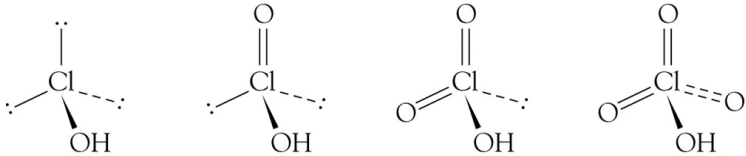
\includegraphics[width=\textwidth]{figures/k17s471Cl.png}
\end{flashcard}

\begin{flashcard}[Reaktion]{Angiv den reaktion der finder sted n�r chlorgas opl�ses i vand}
\ce{Cl2 + H2O <=> H+ + Cl- + HClO}
\end{flashcard}

\begin{flashcard}[Fremstilling]{Hvordan fremstilles perchlorat?}
\ce{3Cl2 + 6NaOH -> NaClO3 + 5NaCl(s) + 3H2O}\\ \vspace{7pt}
\ce{4KClO3(l) ->[\text{$\Delta$}] KCl(s) + 3KClO4(s)}
\end{flashcard}

\begin{flashcard}[Anvendelse]{Angiv reaktionen der finder sted n�r en faststof l�fteraket affyres}
\ce{6NH4ClO4 + 8Al -> 4Al2O3 + 3N2 + 3Cl2 + 12H2O(g)}
\end{flashcard}